\documentclass[lettersize,journal]{IEEEtran}
\usepackage{amsmath,amsfonts}
\usepackage{amsthm}
\usepackage{algorithmic}
\usepackage[ruled,vlined,linesnumbered]{algorithm2e}
\usepackage{array}
\usepackage[font=normalsize,labelfont=sf,textfont=sf]{subfig}
\usepackage{textcomp}
\usepackage{tcolorbox}
\usepackage{stfloats}
\usepackage{url}
\usepackage{verbatim}
\usepackage{graphicx}
\usepackage{cite}
\usepackage{tabularx}
\usepackage{multirow}
\usepackage{colortbl}
\usepackage{xcolor}
\usepackage{enumitem}
\usepackage{xspace}
\usepackage{makecell}  
\usepackage{hhline} 
\usepackage{tabularray}
\usepackage{subcaption}
\hyphenation{op-tical net-works semi-conduc-tor IEEE-Xplore}
% updated with editorial comments 8/9/2021

\renewcommand{\algorithmicrequire}{\textbf{Input:}}
\renewcommand{\algorithmicensure}{\textbf{Output:}}
% \newtheorem{thm}{Theorem}[section]
% \newtheorem{lem}[thm]{Lemma}
% \newtheorem{Def}[thm]{Definition}
% \newtheorem{cor}[thm]{Corollary}
% \newtheorem{prop}[thm]{Proposition}
% \newtheorem{con}[thm]{Conjecture}
% \newtheorem{exa}[thm]{Example}
% \newtheorem{rem}[thm]{Remark}
% \newtheorem{sta}[thm]{Statement}
% \newtheorem{cla}{Claim}
% \newtheorem{prob}[thm]{Problem}
% \newtheorem{que}[thm]{Question}
%\newtheorem{definition}{Definition}


\newtheoremstyle{boldstyle} % 样式名称
  {12pt}                   % 上方空白（例如 12pt）
  {12pt}                   % 下方空白（例如 12pt）
  {\itshape}               % 正文字体
  {}                       % 缩进
  {\bfseries}              % 标题字体（加粗）
  {.}                      % 标点符号
  { }                      % 标题后空白
  {}                       % 自定义标签

\theoremstyle{boldstyle}   % 应用样式

% 定义所有定理环境
\newtheorem{thm}{Theorem}%[section]
\newtheorem{lem}[thm]{Lemma}
\newtheorem{Def}[thm]{Definition}
\newtheorem{cor}[thm]{Corollary}
\newtheorem{prop}[thm]{Proposition}
\newtheorem{con}[thm]{Conjecture}
\newtheorem{exa}[thm]{Example}
\newtheorem{rem}[thm]{Remark}
\newtheorem{sta}[thm]{Statement}
\newtheorem{cla}{Claim}
\newtheorem{prob}[thm]{Problem}
\newtheorem{que}[thm]{Question}

% 自定义证明环境
\newenvironment{pf}[1][Proof]{\noindent\textbf{#1.} }{\hfill\rule{1mm}{2mm}}
\def\theequation{\thesection.\arabic{equation}}
\makeatletter \@addtoreset{equation}{section} \makeatother

\newcommand{\ksx}[1]{\textcolor{purple}{\leavevmode ksx: #1}}
\newcommand{\sxl}[1]{\textcolor{blue}{\leavevmode sxl: #1}}

\newcommand*{\tool}{{\textsc{UP-GDN}}\xspace}


\newcommand{\code}[1]{{\fontfamily{cmtt}\fontseries{m}\fontshape{n}\selectfont\small{#1}}}

\newcommand{\revise}[1]{\textcolor{blue}{#1}}


% Define a custom macro for the highlighted box
\newtcolorbox{answerBox}[1][]{colback=gray!10,    % Background color
   colframe=gray!10,   % Border color
   boxrule=0.2mm,      % Border thickness
   arc=0.5mm,            % Rounded corners
   width=\columnwidth,   % Box width
   left=0.2mm,           % Left padding
   right=0.2mm,          % Right padding
   top=0.2mm,            % Top padding
   bottom=0.2mm,         % Bottom padding
   #1}

\begin{document}

\title{Uncertainty-Aware Probabilistic Graph Diagnosis for Interconnection Networks}
\author{
Xueli~Sun, Shuangxiang~Kan$^{*}$, Jianxi~Fan, Weibei~Fan, Jin~Qi, Zhenjiang~Dong
\noindent\thanks{This work is supported by the National Natural Science Foundation of China (Nos.62402241, 62372248, 62272244), the Natural Science Foundation of the Jiangsu Higher Education Institutions of China (No.24KJD520006), Natural Science Research Start-up Foundation of Recruiting Talents of Nanjing University of Posts and Telecommunications (No.NY223189), Natural Science Foundation of Jiangsu Province (No.BK20200753), Key Program of Natural Science Foundation of Jiangsu under (24KJA520006), and the Natural Science Foundation for Excellent Young Scholars of Jiangsu Province under Grant (BK20250143).
}
\thanks{X. Sun and J. Qi are with the College of Internet of Things, Nanjing University of Posts and Telecommunications, Nanjing 210003, China, S. Kan$^{*}$ (corresponding author) is with the University of New South Wales, Sydney, Australia (e-mail: shuangxiangkan@outlook.com), J. Fan is with the College of Computer, Soochow University, Suzhou 215006, China, W. Fan and Z. Dong are with the College of Computer, Nanjing University of Posts and Telecommunications, Nanjing 210003, China. }
\thanks{E-mail: sunxueli@njupt.edu.cn.}
}
% <-this % stops a space}
% \author{
% \IEEEauthorblockA{Xueli Sun}\\
% \textit{Nanjing University of Posts and Telecommunications}\\
% Nanjing, China\\
% \IEEEauthorblockA{Shuangxiang Kan}\\
% \textit{University of New South Wales}\\
% Sydney, Australia\\
% shuangxiang.kan@unsw.edu.au
% }


% % The paper headers
% \markboth{Journal of \LaTeX\ Class Files,~Vol.~14, No.~8, August~2021}%
% {Shell \MakeLowercase{\textit{et al.}}: A Sample Article Using IEEEtran.cls for IEEE Journals}

% \IEEEpubid{0000--0000/00\$00.00~\copyright~2021 IEEE}
% Remember, if you use this you must call \IEEEpubidadjcol in the second
% column for its text to clear the IEEEpubid mark.

\maketitle

\begin{abstract}
The reliability of large-scale interconnection networks is critical for high-performance computing and cloud infrastructures. System-level diagnosis identifies faulty processors from mutual testing outcomes, but probabilistic diagnosis remains challenging because the observed syndromes are noisy, diagnostic reliability parameters may be unknown or time-varying, and a hard fault/non-fault decision provides little information about diagnostic confidence. This paper presents \tool, an uncertainty-aware probabilistic graph diagnosis framework for the probabilistic PMC model. Instead of treating diagnosis as ordinary node classification, \tool estimates calibrated node-wise fault posterior probabilities, quantifies predictive uncertainty, and ranks suspicious processors for risk-aware maintenance. The framework jointly exploits coarse-grained statistical summaries and fine-grained multi-round syndrome observations through reliability-aware graph message passing. To improve robustness, \tool is trained over a distribution of probabilistic PMC parameters and can adapt to unseen diagnostic reliability conditions.
Experiments on representative interconnection networks show that \tool maintains high diagnostic performance under different fault rates, network scales, and parameter shifts. Beyond accuracy, \tool achieves better calibration and top-$k$ fault localization than classification-oriented graph neural baselines, demonstrating its effectiveness for dependable probabilistic fault diagnosis.
\end{abstract}

\begin{IEEEkeywords}
Fault tolerance, interconnection networks, probabilistic fault diagnosis, graph neural networks, uncertainty estimation
\end{IEEEkeywords}

\section{Introduction}

Large-scale parallel and distributed systems rely on interconnection networks to coordinate thousands or even millions of processing units. Faults in such systems may corrupt data, interrupt services, and trigger cascading failures. System-level diagnosis offers a classical and effective paradigm for identifying faulty processors through mutual tests among adjacent processors~\cite{pmc67,kavianpour2002comparative}. In the PMC model, a processor tests its neighbors and the collection of test outcomes, called a syndrome, is used to infer the faulty processors in the system.

Most classical diagnosis studies assume deterministic testing behavior and derive diagnosability conditions from specific topological properties~\cite{wang1994diagnosability,zhu2016diagnosis,chang2020conditional,tang2024connectivity}. These results are theoretically important, but they become difficult to use in modern systems where diagnostic observations are noisy and the same test may produce different outcomes under different operating conditions. The probabilistic PMC model addresses this issue by assigning probabilities to test outcomes~\cite{blough1989efficient,sun2023probabilistic}. In this model, the reliability of a test is controlled by parameters such as $\gamma$ and $\beta$, which characterize the probability of observing agreement or disagreement under different node states. However, probabilistic diagnosis is computationally challenging because the true fault set is a latent variable and the likelihood must be evaluated over an exponentially large search space.

Graph neural networks (GNNs) provide a promising tool for scalable diagnosis because interconnection networks are naturally represented as graphs and fault evidence is strongly local. A straightforward solution is to transform probabilistic diagnosis into node-level binary classification and train a GNN to predict whether each processor is faulty. Although effective in simple settings, this classification-oriented formulation has three important limitations. First, a hard label does not reveal how confident the diagnosis is, even when several nodes have ambiguous evidence. Second, the output probability of a neural classifier is often poorly calibrated; a score of $0.9$ does not necessarily mean that the node is faulty with probability $0.9$. Third, existing learning-based formulations usually assume fixed diagnostic parameters during training and testing, while the true reliability of tests may be unknown, heterogeneous, or shifted by workload and environmental changes.

This paper takes a different view. We formulate probabilistic fault diagnosis as an uncertainty-aware posterior inference problem rather than a hard classification problem. Given a graph and multi-round probabilistic syndromes, our goal is to estimate the node-wise fault posterior probability $P(z_u=1\mid \mathbb{S},G)$, quantify the uncertainty of this estimate, and provide a ranked list of suspicious processors for risk-aware inspection. This formulation better matches the probabilistic nature of the PMC model: when the evidence is strong, the model should make confident predictions; when the evidence is conflicting or the testing environment is unreliable, the model should explicitly expose uncertainty instead of producing overconfident labels.

To this end, we propose \tool, an uncertainty-aware probabilistic graph diagnosis framework. \tool combines two complementary sources of diagnostic evidence. The first source is a set of interpretable statistical summaries, such as match ratio, mismatch ratio, and neighborhood disagreement variation. These features provide stable local evidence and support explanation. The second source is the raw multi-round syndrome sequence on each edge, which preserves fine-grained stochastic patterns that may be lost after simple aggregation. A reliability-aware graph inference module then propagates evidence across the topology while learning how much each edge-level observation should be trusted. Finally, a posterior diagnosis head produces calibrated fault probabilities and uncertainty scores. To avoid overfitting to a single diagnostic environment, \tool is trained with randomized probabilistic PMC parameters and evaluated under both seen and unseen parameter settings.

In summary, this paper makes the following contributions:
\begin{itemize}[leftmargin=*, itemsep=1pt, parsep=0pt, topsep=1pt]
    \item We formulate probabilistic PMC diagnosis as a posterior inference problem that estimates calibrated node-wise fault probabilities, uncertainty scores, and top-$k$ suspicious processors instead of only hard fault labels.
    \item We propose \tool, a reliability-aware graph diagnosis framework that fuses statistical diagnostic summaries with raw multi-round syndrome observations for probabilistic evidence propagation.
    \item We introduce parameter-robust training for unknown or varying probabilistic PMC reliability parameters, enabling diagnosis under diagnostic reliability shifts.
    \item We conduct experiments on representative interconnection networks and evaluate not only accuracy, precision, recall, and F1-score, but also calibration quality, ranking effectiveness, and robustness to parameter shifts.
\end{itemize}
\section{Preliminaries}\label{preliminaries}

% \subsection{Interconnection Networks}
An interconnection network is modeled as an undirected graph $G=(V,E)$, where each node $u\in V$ represents a processor or server and each edge $(u,v)\in E$ represents a communication or testing relation. Each node has an unknown binary state $z_u\in\{0,1\}$, where $z_u=0$ denotes a fault-free node and $z_u=1$ denotes a faulty node. The true fault set is $F=\{u\in V\mid z_u=1\}$. Standard graph-theoretic notation follows~\cite{bondy1976graph}.

\subsection{Probabilistic PMC Model}
In the probabilistic PMC model, adjacent nodes test each other and produce diagnostic outcomes. For an undirected edge $(u,v)\in E$, we use $S_{u\rightarrow v}\in\{0,1\}$ to denote the outcome when node $u$ tests node $v$, where $S_{u\rightarrow v}=0$ indicates a match and $S_{u\rightarrow v}=1$ indicates a mismatch. Mutual testing on edge $(u,v)$ therefore produces two directed outcomes, $S_{u\rightarrow v}$ and $S_{v\rightarrow u}$. The conditional distribution of a directed outcome depends on the states of the two endpoints:
\begin{equation}
P(S_{u\rightarrow v}=s\mid z_u,z_v)=
\begin{cases}
1, & s=0, z_u=0,z_v=0,\\
\gamma, & s=1, z_u\ne z_v,\\
1-\gamma, & s=0, z_u\ne z_v,\\
\beta, & s=0, z_u=1,z_v=1,\\
1-\beta, & s=1, z_u=1,z_v=1.
\end{cases}
\label{eq:prob_pmc}
\end{equation}
Here $\gamma$ is the probability that a test involving one faulty and one fault-free node yields a mismatch, and $\beta$ is the probability that two faulty nodes yield a match. Typically, $\gamma$ is close to $1$ and $\beta$ is close to $0$, but in practice these parameters may be unknown or may vary across systems and operating conditions.

Because a single probabilistic test can be unreliable, we consider $T$ repeated observations in each direction of an edge:
\begin{equation*}
\mathbb{S}_{u\rightarrow v}=\{S_{u\rightarrow v}^{(1)},S_{u\rightarrow v}^{(2)},\ldots,S_{u\rightarrow v}^{(T)}\}.
\end{equation*}
The complete multi-round syndrome is $\mathbb{S}=\{\mathbb{S}_{u\rightarrow v},\mathbb{S}_{v\rightarrow u}\mid (u,v)\in E\}$.

\subsection{Posterior Diagnosis Objective}
Classical probabilistic diagnosis seeks a fault set that maximizes the likelihood of the observed syndrome:
\begin{equation*}
\hat{F}=\arg\max_{F'\subseteq V} P(\mathbb{S}\mid F').
\end{equation*}
This objective is difficult to solve exactly for large networks because the search space grows exponentially with $|V|$. Moreover, a single estimated set $\hat{F}$ does not convey diagnostic confidence.

We therefore formulate diagnosis as node-wise posterior inference:
\begin{equation*}
p_u=P(z_u=1\mid \mathbb{S},G), \quad u\in V.
\end{equation*}
The output $p_u$ is used both for binary diagnosis and for ranking suspicious processors. A well-calibrated posterior should satisfy the following intuition: among nodes assigned probability close to $0.8$, approximately $80\%$ should be faulty. This property is important for maintenance decisions because it allows operators to distinguish highly reliable alarms from ambiguous cases that require additional testing.

\section{Methodology}
\label{sec:methodology}

\begin{figure*}[h]
    \centering
    \includegraphics[width=0.9\textwidth]{Figures/framework.pdf}
    \caption{\tool framework. The proposed model first estimates node-wise fault posterior probabilities with a GNN and then refines uncertain predictions by checking local syndrome consistency under the probabilistic PMC model.}
    \label{fig:framework}
\end{figure*}

\subsection{Overview}

Building on the probabilistic PMC formulation, this section presents the design of \tool for uncertainty-aware graph diagnosis. The method consists of four stages. First, multi-round mutual-test outcomes are summarized into simple node-level diagnostic features. Second, a GNN posterior estimator produces a fault probability for each processor. Third, high-confidence predictions are directly assigned to fault-free or faulty classes, while uncertain predictions are selected for further checking. Finally, selected predictions are refined by evaluating their local syndrome consistency with high-confidence neighbors under the probabilistic PMC model. In this design, the GNN component serves as an initial posterior estimator, and the key step of \tool is the local posterior refinement that uses the probabilistic PMC likelihood.

\subsection{Diagnostic Feature Construction}

To keep the learning component simple, \tool uses node-level diagnostic summaries as input features. The raw multi-round syndrome observations are not treated as additional neural features; they are retained for the posterior refinement step described later.

For each edge $(u,v)$, mutual testing provides two directed outcomes in each round: $S_{u\rightarrow v}^{(t)}$ and $S_{v\rightarrow u}^{(t)}$. We aggregate the bidirectional match and mismatch counts on edge $(u,v)$ as
\begin{equation*}
c_{uv}=\sum_{t=1}^{T}\left(\mathbb{I}[S_{u\rightarrow v}^{(t)}=0]+\mathbb{I}[S_{v\rightarrow u}^{(t)}=0]\right),
\end{equation*}
\begin{equation*}
m_{uv}=\sum_{t=1}^{T}\left(\mathbb{I}[S_{u\rightarrow v}^{(t)}=1]+\mathbb{I}[S_{v\rightarrow u}^{(t)}=1]\right),
\end{equation*}
where $c_{uv}+m_{uv}=2T$. The bidirectional mismatch ratio is denoted by $r_{uv}=m_{uv}/(2T)$.

\noindent\textbf{Node features.}
For each node $u$, \tool constructs a three-dimensional node feature vector
\begin{equation*}
\mathbf{x}_u=[f_1(u),f_2(u),f_3(u)]^T.
\end{equation*}
We intentionally remove node degree from the feature vector because the considered interconnection networks are regular under a fixed topology, making degree non-discriminative for diagnosis.

\noindent\textit{Average match ratio.}
The first component is the average match ratio:
\begin{equation*}
f_1(u)=\frac{\sum_{v\in N(u)}c_{uv}}{2T|N(u)|}.
\end{equation*}
This feature captures the extent to which node $u$ agrees with its neighborhood across repeated mutual tests.

\noindent\textit{Average mismatch ratio.}
The second component is the average mismatch ratio:
\begin{equation*}
f_2(u)=\frac{\sum_{v\in N(u)}m_{uv}}{2T|N(u)|}.
\end{equation*}
Under the probabilistic PMC model, mismatches provide direct evidence that two adjacent nodes are likely in different states. Therefore, $f_2(u)$ gives a coarse suspicion signal for node $u$ relative to its neighborhood.

\noindent\textit{Mismatch dispersion.}
The third component is the dispersion of edge-level mismatch ratios:
\begin{equation*}
f_3(u)=\sqrt{\frac{1}{|N(u)|}\sum_{v\in N(u)}(r_{uv}-f_2(u))^2}.
\end{equation*}
This feature distinguishes different local disagreement patterns that may have the same average mismatch ratio. For example, disagreement concentrated on one incident edge may suggest that the neighbor on that edge is suspicious, whereas disagreement distributed across many incident edges may indicate broader uncertainty around $u$ or a noisier local syndrome pattern.

\subsection{GNN Posterior Estimator}

Given the node features constructed above, \tool uses a standard message-passing GNN to estimate node-wise fault posterior probabilities. The posterior refinement procedure is not tied to a specific GNN backbone; it can be instantiated with common graph encoders such as mean aggregation, GCN, GraphSAGE, or graph attention.

The initial node representation is
\begin{equation*}
\mathbf{h}_u^{(0)}=\phi_x(\mathbf{x}_u),
\end{equation*}
where $\phi_x(\cdot)$ is an MLP. At layer $\ell$, node $u$ aggregates representations from its graph neighbors:
\begin{equation*}
\mathbf{h}_u^{(\ell+1)}=
\sigma\left(\mathbf{W}_{s}^{(\ell)}\mathbf{h}_u^{(\ell)}
+ \sum_{v\in N(u)} \alpha_{uv}^{(\ell)}
\mathbf{W}_{n}^{(\ell)}\mathbf{h}_v^{(\ell)}\right),
\end{equation*}
where $\alpha_{uv}^{(\ell)}$ denotes the normalized aggregation weight. It can be instantiated as a uniform mean-aggregation weight or as a learned attention weight, depending on the selected backbone.

After $L$ graph layers, the prediction head produces a fault posterior score:
\begin{equation*}
l_u=\mathbf{w}_{p}^{T}\mathbf{h}_u^{(L)}+b_p,\quad
\hat{p}_u=\sigma(l_u).
\end{equation*}
Thus, the GNN provides an initial posterior estimate. Instead of directly converting all posterior scores into hard labels, \tool passes $\hat{p}_u$ to the confidence-aware decision and posterior refinement stages described next.

\subsection{Probability-Based Diagnostic Decision}

The posterior score $\hat{p}_u$ is first converted to a preliminary diagnosis through a confidence-aware decision rule. Let $\theta_-$ and $\theta_+$ be two probability thresholds that define the low-confidence interval around the decision boundary, with $\theta_-<\theta_+$. We define
\begin{align*}
\mathcal{V}_{0} &= \{u\in V: \hat{p}_u\le \theta_-\},\\
\mathcal{V}_{1} &= \{u\in V: \hat{p}_u\ge \theta_+\},\\
\mathcal{V}_{a} &= \{u\in V: \theta_-<\hat{p}_u<\theta_+\},
\end{align*}
where $\mathcal{V}_{0}$ and $\mathcal{V}_{1}$ are preliminarily assigned as fault-free and faulty nodes, respectively, and $\mathcal{V}_{a}$ contains nodes near the decision boundary. The concrete threshold values are specified in the experimental setup.

Nodes in $\mathcal{V}_{0}$ and $\mathcal{V}_{1}$ are assigned direct diagnostic labels:
\begin{equation*}
\hat{z}_u=
\begin{cases}
0, & u\in \mathcal{V}_{0},\\
1, & u\in \mathcal{V}_{1}.
\end{cases}
\end{equation*}
However, a large posterior score does not always imply a reliable prediction under shifted or noisy PMC observations. The GNN may produce overconfident but incorrect predictions. Therefore, \tool does not select refinement candidates only from $\mathcal{V}_{a}$. For each node, we define the prediction confidence as
\begin{equation*}
c_u=\max\{\hat{p}_u,1-\hat{p}_u\}.
\end{equation*}
Let $\mathcal{T}_{q}^{0}$ and $\mathcal{T}_{q}^{1}$ denote the least-confident top-$q$ fraction of nodes in $\mathcal{V}_{0}$ and $\mathcal{V}_{1}$ according to $c_u$, respectively. The posterior refinement candidate set is
\begin{equation*}
\mathcal{V}_{r}=\mathcal{V}_{a}\cup\mathcal{T}_{q}^{0}\cup\mathcal{T}_{q}^{1}.
\end{equation*}
This selection keeps boundary-region ambiguous nodes while also allowing low-confidence predictions within each preliminary class to be checked against local syndrome evidence.

\subsection{Posterior Refinement via Local Syndrome Consistency}
\label{subsec:posterior_calibration}

For a refinement candidate $u\in\mathcal{V}_{r}$, the GNN posterior alone may be insufficient for a reliable decision. Instead of calibrating all nodes globally, \tool refines selected predictions by checking whether each candidate state of $u$ is consistent with the observed mutual-test syndromes around reliable neighboring nodes.

Let
\begin{equation*}
\mathcal{H}_u=N(u)\cap((\mathcal{V}_{0}\cup\mathcal{V}_{1})\setminus\mathcal{V}_{r})
\end{equation*}
be the set of reference neighbors of $u$. Nodes selected for refinement are excluded from this reference set because their preliminary labels require further checking. For each $v\in\mathcal{H}_u$, its provisional label is fixed as $\hat{z}_v=0$ if $v\in\mathcal{V}_{0}$ and $\hat{z}_v=1$ if $v\in\mathcal{V}_{1}$.

\tool then evaluates two hypotheses for node $u$: $z_u=1$ and $z_u=0$. Under a candidate state $h\in\{0,1\}$, the local syndrome likelihood is
\begin{equation*}
\mathcal{L}_u(h)=
\prod_{v\in\mathcal{H}_u}\prod_{t=1}^{T}
P(S_{u\rightarrow v}^{(t)}\mid h,\hat{z}_v)
P(S_{v\rightarrow u}^{(t)}\mid \hat{z}_v,h),
\end{equation*}
where the conditional probabilities follow the probabilistic PMC model. This likelihood measures how well the collected bidirectional syndrome on edges incident to high-confidence neighbors agrees with the assumed state of $u$.

The refined posterior combines the GNN score with this local consistency evidence:
\begin{equation*}
\tilde{p}_u=
\frac{\hat{p}_u\mathcal{L}_u(1)}
{\hat{p}_u\mathcal{L}_u(1)+(1-\hat{p}_u)\mathcal{L}_u(0)}.
\end{equation*}
If the observed mutual-test outcomes are much more consistent with the faulty hypothesis, $\tilde{p}_u$ increases; if they are more consistent with the fault-free hypothesis, $\tilde{p}_u$ decreases. When $\mathcal{H}_u$ is empty or the two hypotheses produce similar likelihoods, the node remains uncertain and the refined posterior stays close to the original GNN score.

For refinement candidates, the final diagnosis is determined by the refined posterior and a decision threshold $\theta_c$:
\begin{equation*}
\hat{z}_u=\mathbb{I}[\tilde{p}_u\ge \theta_c],\quad u\in\mathcal{V}_{r}.
\end{equation*}
For nodes not selected into $\mathcal{V}_{r}$, the preliminary labels from the previous decision stage are retained.

\noindent\textbf{Example.}
Consider node $u=000$ in a three-dimensional hypercube $Q_3$, whose neighbors are $001$, $010$, and $100$. Suppose $u$ is selected into $\mathcal{V}_{r}$ because its posterior is near the decision boundary or because it is among the least-confident nodes in its preliminary class. Suppose further that $001$ and $100$ are reliable fault-free reference nodes, while $010$ is also selected for refinement. The refinement step uses only $\mathcal{H}_u=\{001,100\}$ and ignores $010$.

Assume first that $T=5$ bidirectional tests are observed as
\begin{equation*}
\begin{aligned}
\mathbf{s}_{u,001}&=1111111100,\\
\mathbf{s}_{u,100}&=1111101111,
\end{aligned}
\end{equation*}
where each sequence concatenates the outcomes from $u$ to the neighbor and from the neighbor to $u$. Both edges contain mostly mismatches. Since $001$ and $100$ are treated as fault-free references, these observations are more consistent with the hypothesis $z_u=1$ than with $z_u=0$. Therefore, $\mathcal{L}_u(1)>\mathcal{L}_u(0)$ and the refined posterior $\tilde{p}_u$ moves toward the faulty class. Conversely, if the two sequences were mostly matches, the same calculation would make $\mathcal{L}_u(0)$ larger and move $\tilde{p}_u$ toward the fault-free class. Thus, ambiguous nodes are not decided only by their GNN score, but by whether their candidate states are consistent with reliable neighboring syndromes.

\section{Experiment}
\label{sec:simulation}

This section evaluates the proposed \tool framework under the probabilistic PMC setting. The evaluation is organized around three research questions:
\begin{itemize}[leftmargin=*, itemsep=1pt, parsep=0pt, topsep=1pt]
    \item \textbf{RQ1:} How effective is \tool compared with existing diagnosis methods?
    \item \textbf{RQ2:} How does \tool perform under different fault rates?
    \item \textbf{RQ3:} How do diagnostic features, posterior refinement, and GNN backbones affect \tool?
\end{itemize}

\subsection{Experimental Setup}

\noindent \textbf{Network topologies.}
We evaluate all methods on three representative interconnection topologies. The first topology is the hypercube $Q_n$, where each node is represented by an $n$-bit binary string and adjacent nodes differ in exactly one bit. The second topology is the $k$-ary $n$-cube $Q_k^n$, where each node is represented by an $n$-tuple over $\{0,1,\ldots,k-1\}$ and two nodes are adjacent if they differ by one modulo $k$ in exactly one dimension. The third topology is the augmented $k$-ary $n$-cube $AQ_{n,k}$, which extends $Q_k^n$ with additional augmented edges to provide higher connectivity. These three topologies cover different degrees, local connectivity patterns, and diagnostic evidence densities.

\noindent \textbf{Fault and syndrome generation.}
For each topology, faulty nodes are sampled according to a specified fault rate. Given the fault state of each node, directed test outcomes are generated according to the probabilistic PMC model. Each adjacent pair is tested in both directions, and each directed test is repeated for $T$ rounds unless otherwise specified. The proposed method uses the multi-round syndrome observations, while the rule-based baseline is evaluated using the last collected syndrome.

\noindent \textbf{Baselines.}
To the best of our knowledge, \tool is the first neural-network-based method for system-level probabilistic PMC diagnosis model. Therefore, we compare it with a representative traditional method, Clustered-PMC, the probabilistic clustered-fault diagnosis algorithm based on local factions and threshold $k=3$~\cite{sun2023probabilistic}. Since Clustered-PMC takes a single PMC syndrome as input, we apply it to the last collected syndrome in each test instance. Clustered-PMC is directly evaluated on the validation or test instances without training.

\noindent \textbf{Metrics.}
For binary diagnosis, we report accuracy, precision, recall, and F1-score. Since \tool produces posterior fault probabilities, we also report Brier score and expected calibration error (ECE) to evaluate probability quality. Lower Brier score and lower ECE indicate better calibrated posterior estimates.

\noindent \textbf{Implementation details.}
In RQ1 and RQ2, the GNN posterior estimator is instantiated with GraphSAGE. In RQ3, we use GraphSAGE for the feature and posterior-refinement studies, and separately compare GCN, GraphSAGE, and GAT in the backbone study. The default decision threshold for calibrated posterior diagnosis is $\theta_c=0.5$. The least-confident top-$q$ fraction in each preliminary class is selected for posterior refinement, with $q=10\%$ by default. The concrete values of $T$, fault rates, graph sizes, training epochs, hidden dimensions, and optimization settings are reported together with the corresponding experiments.

\noindent \textbf{Experimental environment.}
All experiments are conducted on a workstation equipped with an Intel Core i7-14700KF CPU and an NVIDIA GeForce RTX 5060 Ti GPU with 16 GB memory. The implementation uses Python 3.13, PyTorch 2.12.0 with CUDA 13.0 support, and NumPy 2.4.6. 

\subsection{RQ1: Overall Diagnostic Effectiveness}
\label{subsec:rq1}

RQ1 evaluates whether \tool can accurately diagnose faulty processors under the probabilistic PMC model. We compare \tool with Clustered-PMC on the three topologies described above. In the GPU-scale setting, we evaluate three larger instances from each topology family: $Q_6$, $Q_8$, $Q_{10}$, $Q_8^2$, $Q_6^3$, $Q_5^4$, $AQ_{2,8}$, $AQ_{3,6}$, and $AQ_{4,5}$. The fault rate is fixed to $30\%$, and each result is averaged over three independent runs.

For each topology instance and each run, we generate $200$ training samples and $100$ test samples with $T=2$ rounds of mutual testing. Unless otherwise stated, the probabilistic PMC parameters are sampled from $\gamma \sim U(0.7, 1.0)$ and $\beta \sim U(0.0, 0.3)$. The posterior estimator uses a two-layer GraphSAGE backbone with hidden dimension $64$, and is trained for $100$ epochs on GPU. The refinement candidate ratio is fixed to $q=10\%$. To improve training throughput for the GPU-scale setting, we use mini-batches of $16$ samples together with CUDA mixed-precision training.

\begin{table}[h]
\centering
\caption{RQ1 diagnostic performance in the GPU-scale setting.}
\label{tab:rq1_effectiveness}
\resizebox{0.48\textwidth}{!}{%
\begin{tabular}{|c|c|c|c|c|c|c|}
\hline
\textbf{Topology} & \textbf{Method} & \textbf{Accuracy} & \textbf{Precision} & \textbf{Recall} & \textbf{F1} & \textbf{Brier} \\
\hline
$Q_6$ & Clustered-PMC & 0.8401 & 0.9962 & 0.4616 & 0.5959 & 0.1599 \\
$Q_6$ & \tool & 0.9999 & 0.9998 & 0.9998 & 0.9998 & 0.0001 \\
\hline
$Q_8$ & Clustered-PMC & 0.8100 & 1.0000 & 0.3682 & 0.4934 & 0.1900 \\
$Q_8$ & \tool & 1.0000 & 1.0000 & 1.0000 & 1.0000 & 0.0000 \\
\hline
$Q_{10}$ & Clustered-PMC & 0.7943 & 1.0000 & 0.3139 & 0.4329 & 0.2057 \\
$Q_{10}$ & \tool & 1.0000 & 1.0000 & 1.0000 & 1.0000 & 0.0000 \\
\hline
$Q_8^2$ & Clustered-PMC & 0.8804 & 0.9781 & 0.6130 & 0.7289 & 0.1196 \\
$Q_8^2$ & \tool & 0.9991 & 0.9995 & 0.9974 & 0.9984 & 0.0008 \\
\hline
$Q_6^3$ & Clustered-PMC & 0.8415 & 0.9984 & 0.4739 & 0.6097 & 0.1585 \\
$Q_6^3$ & \tool & 0.9999 & 0.9998 & 0.9997 & 0.9997 & 0.0001 \\
\hline
$Q_5^4$ & Clustered-PMC & 0.8124 & 1.0000 & 0.3762 & 0.5076 & 0.1876 \\
$Q_5^4$ & \tool & 1.0000 & 0.9999 & 0.9999 & 1.0000 & 0.0000 \\
\hline
$AQ_{2,8}$ & Clustered-PMC & 0.8422 & 0.9914 & 0.4705 & 0.5991 & 0.1578 \\
$AQ_{2,8}$ & \tool & 1.0000 & 1.0000 & 1.0000 & 1.0000 & 0.0000 \\
\hline
$AQ_{3,6}$ & Clustered-PMC & 0.7969 & 0.9967 & 0.3250 & 0.4431 & 0.2031 \\
$AQ_{3,6}$ & \tool & 1.0000 & 1.0000 & 1.0000 & 1.0000 & 0.0000 \\
\hline
$AQ_{4,5}$ & Clustered-PMC & 0.7602 & 0.9967 & 0.2027 & 0.2948 & 0.2398 \\
$AQ_{4,5}$ & \tool & 1.0000 & 1.0000 & 1.0000 & 1.0000 & 0.0000 \\
\hline
\end{tabular}%
}
\vspace{1mm}
\end{table}

Table~\ref{tab:rq1_effectiveness} shows that \tool consistently improves recall and F1-score over Clustered-PMC while maintaining high precision. Across all nine GPU-scale topologies, \tool achieves near-perfect diagnosis, with F1 scores between $0.9984$ and $1.0000$ and Brier scores between $0.0000$ and $0.0008$. In contrast, Clustered-PMC remains much more conservative: its precision is usually close to one, but its recall drops substantially as the topology becomes larger or more densely augmented, leading to markedly lower F1 scores.

More specifically, on the hypercube family, the F1 score of Clustered-PMC decreases from $0.5959$ on $Q_6$ to $0.4329$ on $Q_{10}$, while \tool remains essentially perfect on all three instances. A similar pattern appears on the augmented $k$-ary family: Clustered-PMC reaches $0.5991$ on $AQ_{2,8}$, drops to $0.4431$ on $AQ_{3,6}$, and further drops to $0.2948$ on $AQ_{4,5}$, whereas \tool maintains an F1 score of $1.0000$ throughout. Even on the comparatively easier $k$-ary case $Q_8^2$, where Clustered-PMC attains its best F1 score of $0.7289$, \tool still improves the F1 score to $0.9984$. These results indicate that the posterior-estimation-and-refinement pipeline is not tied to one specific topology parameterization; instead, it remains highly effective across diverse $(k,n)$ combinations, while the rule-based baseline suffers mainly from low recall and therefore misses a nontrivial portion of faulty processors.

\subsection{RQ2: Performance Under Different Fault Rates}
\label{subsec:rq2_fault_rate}

RQ2 evaluates the robustness of \tool as the number of faulty processors increases. We vary the fault rate and compare \tool with Clustered-PMC under the same syndrome generation setting. This experiment is designed to test whether the posterior-based diagnosis remains effective when local neighborhoods contain more faulty nodes and the observed syndromes become more ambiguous.

In the GPU-scale setting, we use one representative larger instance from each topology family, namely $Q_{10}$, $Q_4^5$, and $AQ_{5,4}$. The fault rate is varied from $10\%$ to $50\%$ in steps of $5\%$, i.e., $\{10\%, 15\%, 20\%, 25\%, 30\%, 35\%, 40\%, 45\%, 50\%\}$. The remaining settings are the same as in RQ1: $T=2$, $\gamma \sim U(0.7, 1.0)$, $\beta \sim U(0.0, 0.3)$, $200$ training samples and $100$ test samples per topology instance, a two-layer GraphSAGE posterior estimator with hidden dimension $64$, $100$ training epochs, and posterior refinement ratio $q=10\%$. Each rate-wise result is averaged over the three topologies and three independent runs per topology.

\begin{table}[h]
\centering
\caption{Diagnostic performance under different fault rates.}
\label{tab:rq2_fault_rate}
\resizebox{0.48\textwidth}{!}{%
\begin{tabular}{|c|c|c|c|c|c|c|}
\hline
\textbf{Fault Rate} & \textbf{Method} & \textbf{Accuracy} & \textbf{Precision} & \textbf{Recall} & \textbf{F1} & \textbf{ECE} \\
\hline
10\% & Clustered-PMC & 0.9268 & 0.9356 & 0.2656 & 0.3631 & -- \\
10\% & \tool & 1.0000 & 1.0000 & 1.0000 & 1.0000 & 0.0000 \\
\hline
15\% & Clustered-PMC & 0.8855 & 0.9533 & 0.2384 & 0.3289 & -- \\
15\% & \tool & 1.0000 & 1.0000 & 1.0000 & 1.0000 & 0.0000 \\
\hline
20\% & Clustered-PMC & 0.8534 & 0.9822 & 0.2679 & 0.3686 & -- \\
20\% & \tool & 1.0000 & 1.0000 & 1.0000 & 1.0000 & 0.0000 \\
\hline
25\% & Clustered-PMC & 0.8073 & 0.9844 & 0.2291 & 0.3263 & -- \\
25\% & \tool & 1.0000 & 1.0000 & 1.0000 & 1.0000 & 0.0000 \\
\hline
30\% & Clustered-PMC & 0.7748 & 0.9867 & 0.2486 & 0.3496 & -- \\
30\% & \tool & 1.0000 & 1.0000 & 1.0000 & 1.0000 & 0.0000 \\
\hline
35\% & Clustered-PMC & 0.7356 & 0.9943 & 0.2438 & 0.3450 & -- \\
35\% & \tool & 1.0000 & 1.0000 & 1.0000 & 1.0000 & 0.0000 \\
\hline
40\% & Clustered-PMC & 0.6949 & 0.9977 & 0.2380 & 0.3398 & -- \\
40\% & \tool & 1.0000 & 1.0000 & 1.0000 & 1.0000 & 0.0000 \\
\hline
45\% & Clustered-PMC & 0.6618 & 0.9952 & 0.2489 & 0.3528 & -- \\
45\% & \tool & 0.9999 & 0.9999 & 0.9999 & 0.9999 & 0.0001 \\
\hline
50\% & Clustered-PMC & 0.6193 & 0.9959 & 0.2389 & 0.3436 & -- \\
50\% & \tool & 0.9998 & 0.9998 & 0.9998 & 0.9998 & 0.0002 \\
\hline
\end{tabular}%
}
\vspace{1mm}
\end{table}

Table~\ref{tab:rq2_fault_rate} shows that \tool remains highly robust as the fault rate increases. From $10\%$ to $40\%$, \tool maintains essentially perfect diagnosis, with accuracy and F1 both equal to $1.0000$ after rounding. Even at the highest tested fault rates of $45\%$ and $50\%$, the performance drop is negligible: the F1 score remains $0.9999$ and $0.9998$, respectively, while the ECE stays below $2.5 \times 10^{-4}$.

By contrast, Clustered-PMC degrades substantially as the fault rate increases. Its accuracy decreases from $0.9268$ at $10\%$ faults to $0.6193$ at $50\%$ faults. More importantly, its recall remains consistently low across all rates, fluctuating only between about $0.23$ and $0.27$, which leads to poor F1 scores in the range of $0.3263$--$0.3686$ for most settings. This behavior indicates that the rule-based baseline is overly conservative under the probabilistic PMC setting: it keeps precision high, but misses many faulty processors once the local syndromes become noisier and more ambiguous. In contrast, the posterior-based diagnosis in \tool degrades much more gracefully and preserves both discrimination and calibration quality over the full fault-rate range.

\subsection{RQ3: Ablation Study}
\label{subsec:rq3_ablation}

RQ3 studies three design questions in \tool. First, we evaluate the contribution of each node feature. Second, we measure the contribution of local syndrome-consistency posterior refinement. Third, we compare different GNN backbones to check whether the framework is tied to a specific graph encoder.

\noindent\textbf{Feature study.}
We first study the node feature design by removing one feature at a time while keeping the GNN backbone and posterior refinement unchanged:
\begin{itemize}[leftmargin=*, itemsep=1pt, parsep=0pt, topsep=1pt]
    \item \textbf{w/o match ratio}: removes the average match ratio from the node features.
    \item \textbf{w/o mismatch ratio}: removes the average mismatch ratio from the node features.
    \item \textbf{w/o dispersion}: removes mismatch dispersion from the node features.
    \item \textbf{full \tool}: uses all diagnostic node features and posterior refinement.
\end{itemize}

In the updated GPU setting, this ablation is conducted on the smaller representative topology instances $Q_6$, $Q_8^2$, and $AQ_{2,8}$ with fault rate $30\%$, $T=2$, $\gamma \sim U(0.7, 1.0)$, and $\beta \sim U(0.0, 0.3)$. For each topology instance and each run, we generate $100$ training samples and $100$ test samples. The posterior estimator uses a two-layer GraphSAGE backbone with hidden dimension $64$ and posterior refinement ratio $q=10\%$. To reduce GPU runtime while keeping the convergence comparison meaningful, we train for $60$ epochs, evaluate every $5$ epochs, and use mini-batches of $16$ samples together with CUDA mixed-precision training. Each variant is averaged over the three topologies and three independent runs per topology.

\begin{table}[h]
\centering
\caption{Node feature ablation with convergence-sensitive metrics.}
\label{tab:rq3_feature}
\resizebox{0.48\textwidth}{!}{%
\begin{tabular}{|c|c|c|c|c|c|}
\hline
\textbf{Variant} & \textbf{Final F1} & \textbf{ECE} & \textbf{Best-F1 Epoch} & \textbf{Epoch to F1 $\geq 0.99$} & \textbf{Mean F1 over Epochs} \\
\hline
w/o match ratio & 0.9984 & 0.0012 & 31.67 & 5.67 & 0.9668 \\
w/o mismatch ratio & 0.9986 & 0.0012 & 31.67 & 4.56 & 0.9736 \\
w/o dispersion & 0.9978 & 0.0020 & 26.67 & 6.22 & 0.9812 \\
full \tool & 0.9985 & 0.0011 & 25.56 & 4.78 & 0.9920 \\
\hline
\end{tabular}%
}
\vspace{1mm}
\end{table}

\begin{table*}[t]
\centering
\caption{Complete topology-wise results for the feature ablation study.}
\label{tab:rq3_feature_detail}
\resizebox{\textwidth}{!}{%
\begin{tabular}{|c|c|c|c|c|c|c|}
\hline
\textbf{Topology} & \textbf{Variant} & \textbf{Final F1} & \textbf{ECE} & \textbf{Best-F1 Epoch} & \textbf{Epoch to F1 $\geq 0.99$} & \textbf{Mean F1 over Epochs} \\
\hline
$Q_6$ & w/o match ratio & 0.9993 & 0.0004 & 18.33 & 5.00 & 0.9363 \\
$Q_6$ & w/o mismatch ratio & 0.9993 & 0.0004 & 13.33 & 3.67 & 0.9617 \\
$Q_6$ & w/o dispersion & 0.9995 & 0.0004 & 18.33 & 3.67 & 0.9700 \\
$Q_6$ & full \tool & 0.9994 & 0.0004 & 18.33 & 1.00 & 0.9990 \\
\hline
$Q_8^2$ & w/o match ratio & 0.9971 & 0.0026 & 56.67 & 7.00 & 0.9800 \\
$Q_8^2$ & w/o mismatch ratio & 0.9974 & 0.0025 & 56.67 & 5.00 & 0.9849 \\
$Q_8^2$ & w/o dispersion & 0.9956 & 0.0041 & 51.67 & 10.00 & 0.9884 \\
$Q_8^2$ & full \tool & 0.9970 & 0.0025 & 46.67 & 8.33 & 0.9810 \\
\hline
$AQ_{2,8}$ & w/o match ratio & 0.9989 & 0.0007 & 20.00 & 5.00 & 0.9841 \\
$AQ_{2,8}$ & w/o mismatch ratio & 0.9990 & 0.0007 & 25.00 & 5.00 & 0.9743 \\
$AQ_{2,8}$ & w/o dispersion & 0.9983 & 0.0014 & 10.00 & 5.00 & 0.9852 \\
$AQ_{2,8}$ & full \tool & 0.9992 & 0.0006 & 11.67 & 5.00 & 0.9959 \\
\hline
\end{tabular}%
}
\vspace{1mm}
\end{table*}

Table~\ref{tab:rq3_feature} shows that all four feature variants still achieve strong diagnosis performance on the smaller topology set, but the differences are now more visible than in the larger-topology setting. The final F1 scores range from $0.9978$ to $0.9986$, and the ECE values lie between $0.0011$ and $0.0020$, indicating that the reduced topology scale makes feature ablations more distinguishable in both discrimination and calibration.

The convergence-sensitive metrics show a clearer advantage for the full feature set. Although removing the mismatch ratio attains the highest final F1 by a small margin ($0.9986$ versus $0.9985$ for the full model), the full model reaches its best F1 substantially earlier on average (epoch $25.56$ versus $31.67$) and achieves the highest mean F1 over evaluated epochs ($0.9920$), indicating better overall training efficiency and stability. Removing dispersion is the weakest variant in final performance, yielding the lowest final F1 ($0.9978$) and the highest ECE ($0.0020$), which suggests that mismatch-dispersion information is important for stable posterior calibration on these smaller topologies. Removing the match ratio also slows convergence and reduces training-phase quality, as reflected by its lower mean F1 over epochs ($0.9668$). The complete topology-wise results are reported in Table~\ref{tab:rq3_feature_detail}. They show that the largest difficulty consistently comes from $Q_8^2$, while $Q_6$ and $AQ_{2,8}$ remain nearly saturated across all feature variants. Overall, these results indicate that the three diagnostic features remain complementary: even when the final diagnosis scores stay high, the complete feature set yields the most balanced combination of convergence speed, stability, and calibration quality.

\noindent\textbf{Posterior refinement study.}
We then isolate the effect of the local syndrome-consistency posterior refinement. The variant without posterior refinement directly thresholds the GNN posterior scores, while the full model applies the refinement step to selected low-confidence predictions.

This study uses the same smaller GPU topology set as the feature ablation, namely $Q_6$, $Q_8^2$, and $AQ_{2,8}$, together with fault rate $30\%$, $100$ training samples, $100$ test samples, $60$ training epochs, evaluation every $5$ epochs, mini-batch size $16$, and CUDA mixed-precision training. The GraphSAGE posterior estimator and all feature settings are kept unchanged so that the only difference is whether the local posterior-refinement step is applied.

\begin{table}[h]
\centering
\caption{Effect of posterior refinement.}
\label{tab:rq3_refinement}
\resizebox{0.48\textwidth}{!}{%
\begin{tabular}{|c|c|c|c|c|c|}
\hline
\textbf{Variant} & \textbf{Accuracy} & \textbf{Precision} & \textbf{Recall} & \textbf{F1} & \textbf{ECE} \\
\hline
w/o posterior refinement & 0.9984 & 0.9982 & 0.9966 & 0.9973 & 0.0020 \\
full \tool & 0.9990 & 0.9986 & 0.9982 & 0.9984 & 0.0012 \\
\hline
\end{tabular}%
}
\vspace{1mm}
\end{table}

\begin{table*}[t]
\centering
\caption{Complete topology-wise results for the posterior refinement study.}
\label{tab:rq3_refinement_detail}
\resizebox{\textwidth}{!}{%
\begin{tabular}{|c|c|c|c|c|c|c|c|c|c|}
\hline
\textbf{Topology} & \textbf{Variant} & \textbf{Accuracy} & \textbf{Precision} & \textbf{Recall} & \textbf{F1} & \textbf{ECE} & \textbf{Best-F1 Epoch} & \textbf{Epoch to F1 $\geq 0.99$} & \textbf{Mean F1 over Epochs} \\
\hline
$Q_6$ & w/o posterior refinement & 0.9992 & 0.9985 & 0.9988 & 0.9986 & 0.0010 & 43.33 & 10.00 & 0.9269 \\
$Q_6$ & full \tool & 0.9997 & 0.9993 & 0.9998 & 0.9996 & 0.0003 & 23.33 & 5.00 & 0.9968 \\
\hline
$Q_8^2$ & w/o posterior refinement & 0.9969 & 0.9972 & 0.9925 & 0.9947 & 0.0039 & 55.00 & 18.33 & 0.9135 \\
$Q_8^2$ & full \tool & 0.9979 & 0.9972 & 0.9958 & 0.9964 & 0.0027 & 56.67 & 8.33 & 0.9674 \\
\hline
$AQ_{2,8}$ & w/o posterior refinement & 0.9993 & 0.9990 & 0.9986 & 0.9988 & 0.0011 & 55.00 & 10.00 & 0.9199 \\
$AQ_{2,8}$ & full \tool & 0.9995 & 0.9992 & 0.9991 & 0.9991 & 0.0005 & 15.00 & 5.00 & 0.9736 \\
\hline
\end{tabular}%
}
\vspace{1mm}
\end{table*}

Table~\ref{tab:rq3_refinement} shows that posterior refinement consistently improves the final diagnosis quality on the smaller topology set. Compared with direct thresholding of the raw GNN posterior, the refinement step raises F1 from $0.9973$ to $0.9984$ and reduces ECE from $0.0020$ to $0.0012$, indicating that the refined posterior is not only more accurate but also better calibrated. The improvement is mainly driven by higher recall, which increases from $0.9966$ to $0.9982$, while precision also improves slightly.

The convergence statistics show an even clearer effect. With posterior refinement, the mean F1 over evaluated epochs increases from $0.9201$ to $0.9793$, and the mean best-F1 epoch moves much earlier, from $51.11$ to $31.67$. This indicates that the refinement step does more than polish the final prediction: it produces a more stable diagnosis trajectory throughout training. On average, the refinement module changes only about $0.82\%$ of node predictions in the final evaluation, yet it yields a measurable gain in both F1 and calibration, which suggests that a small number of carefully selected low-confidence corrections is sufficient to improve overall diagnosis quality. Table~\ref{tab:rq3_refinement_detail} provides the complete topology-wise data and shows that the gain is consistent across all three topologies, with the largest absolute benefit appearing on $Q_8^2$, where refinement improves F1 from $0.9947$ to $0.9964$ and shortens the time to F1 $\geq 0.99$ from $18.33$ to $8.33$ epochs.

\noindent\textbf{Backbone comparison.}
We further instantiate the GNN posterior estimator with different graph encoders while keeping the same diagnostic features and posterior refinement procedure. The reported results are averaged over the three representative topologies.

This comparison uses the same smaller GPU topology set $Q_6$, $Q_8^2$, and $AQ_{2,8}$, with fault rate $30\%$, $100$ training samples, $100$ test samples, $60$ training epochs, evaluation every $5$ epochs, mini-batch size $16$, and CUDA mixed-precision training. All backbones use the same node features and the same posterior-refinement procedure so that the only varying component is the graph encoder.

\begin{table}[h]
\centering
\caption{Comparison of different GNN backbones.}
\label{tab:rq3_backbone}
\resizebox{0.48\textwidth}{!}{%
\begin{tabular}{|c|c|c|c|c|c|}
\hline
\textbf{Backbone} & \textbf{Final F1} & \textbf{ECE} & \textbf{Best-F1 Epoch} & \textbf{Epoch to F1 $\geq 0.99$} & \textbf{Mean F1 over Epochs} \\
\hline
GCN & 0.9977 & 0.0024 & 37.78 & 15.00 & 0.9562 \\
GraphSAGE & 0.9985 & 0.0012 & 35.00 & 6.22 & 0.9630 \\
GAT & 0.9983 & 0.0022 & 45.56 & 12.78 & 0.9401 \\
\hline
\end{tabular}%
}
\vspace{1mm}
\end{table}

\begin{table*}[t]
\centering
\caption{Complete topology-wise results for the backbone comparison study.}
\label{tab:rq3_backbone_detail}
\resizebox{\textwidth}{!}{%
\begin{tabular}{|c|c|c|c|c|c|c|}
\hline
\textbf{Topology} & \textbf{Backbone} & \textbf{Final F1} & \textbf{ECE} & \textbf{Best-F1 Epoch} & \textbf{Epoch to F1 $\geq 0.99$} & \textbf{Mean F1 over Epochs} \\
\hline
$Q_6$ & GCN & 0.9996 & 0.0009 & 28.33 & 15.00 & 0.9589 \\
$Q_6$ & GraphSAGE & 0.9995 & 0.0003 & 13.33 & 3.67 & 0.9700 \\
$Q_6$ & GAT & 0.9997 & 0.0008 & 41.67 & 10.00 & 0.9378 \\
\hline
$Q_8^2$ & GCN & 0.9947 & 0.0050 & 55.00 & 18.33 & 0.9437 \\
$Q_8^2$ & GraphSAGE & 0.9969 & 0.0026 & 53.33 & 10.00 & 0.9234 \\
$Q_8^2$ & GAT & 0.9962 & 0.0044 & 53.33 & 16.67 & 0.9483 \\
\hline
$AQ_{2,8}$ & GCN & 0.9989 & 0.0014 & 30.00 & 11.67 & 0.9659 \\
$AQ_{2,8}$ & GraphSAGE & 0.9990 & 0.0006 & 38.33 & 5.00 & 0.9957 \\
$AQ_{2,8}$ & GAT & 0.9990 & 0.0013 & 41.67 & 11.67 & 0.9341 \\
\hline
\end{tabular}%
}
\vspace{1mm}
\end{table*}

Table~\ref{tab:rq3_backbone} shows that all three graph encoders remain effective, but GraphSAGE provides the best overall tradeoff on the smaller topology set. It attains the highest final F1 ($0.9985$), the lowest ECE ($0.0012$), and the fastest rise to F1 $\geq 0.99$ (epoch $6.22$ on average). GAT reaches a slightly lower final F1 ($0.9983$) and converges more slowly, with the latest best-F1 epoch ($45.56$) and the lowest mean F1 over evaluated epochs ($0.9401$). GCN performs competitively, but its final F1 ($0.9977$) and calibration are both slightly worse than GraphSAGE.

The complete topology-wise results in Table~\ref{tab:rq3_backbone_detail} show that the backbone preference depends somewhat on the topology, but the overall ranking is still stable. GraphSAGE is clearly the fastest-converging choice on all three topologies, and it also yields the best calibrated posterior on each topology. GAT attains the highest final F1 on $Q_6$, but this advantage does not transfer to $Q_8^2$ or $AQ_{2,8}$, and its convergence is consistently slower. GCN is competitive on $Q_6$ and $AQ_{2,8}$, but is weakest on $Q_8^2$.

Tables~\ref{tab:rq3_feature}, \ref{tab:rq3_feature_detail}, \ref{tab:rq3_refinement}, \ref{tab:rq3_refinement_detail}, \ref{tab:rq3_backbone}, and~\ref{tab:rq3_backbone_detail} together show that the complete \tool design is supported by three consistent observations on the smaller topology set. First, the full node-feature set mainly improves convergence stability and calibration rather than dramatically changing the final diagnosis score. Second, posterior refinement yields a clear gain in both F1 and ECE with only a small number of selective prediction changes. Third, among the tested GNN encoders, GraphSAGE offers the most favorable balance of final accuracy, calibration, and training efficiency. Therefore, using GraphSAGE as the default backbone in RQ1 and RQ2 remains justified not only by simplicity, but also by the strongest empirical balance observed in the RQ3 ablation study.

\section{Discussion and Limitations}\label{sec:limitation}

\tool provides an uncertainty-aware framework for probabilistic fault diagnosis, but several limitations remain. First, the current formulation focuses on processor faults and treats edge reliability as a confidence weight for syndrome evidence. A more general model could explicitly diagnose both faulty nodes and faulty links as two coupled latent variables. Second, the training data are generated from simulated probabilistic PMC syndromes. Although simulation is standard in system-level diagnosis, future work should validate the method on traces from real high-performance computing or data-center systems. Third, the current posterior approximation is learned by a neural model and does not provide the same type of worst-case diagnosability guarantee as classical graph-theoretic diagnosis. Combining calibrated learning-based diagnosis with formal diagnosability bounds is an important future direction.

Another limitation is that calibration can degrade under severe out-of-distribution shifts. Parameter-randomized training improves robustness, but it cannot cover all possible operating conditions. In practice, \tool should be used together with monitoring mechanisms that detect when the test environment has shifted beyond the training range. Finally, top-$k$ suspicious-node ranking is useful for maintenance, but the optimal value of $k$ may depend on operational cost, repair budget, and service-level requirements.
\section{Related Work}\label{related-work}

\subsection{System-Level Fault Diagnosis}
System-level diagnosis was introduced by Preparata, Metze, and Chien through the PMC model~\cite{pmc67}. Since then, many studies have investigated diagnosability, conditional diagnosability, and diagnosis algorithms for specific interconnection networks~\cite{wang1994diagnosability,zhu2016diagnosis,chang2020conditional,tang2024connectivity}. These works provide rigorous theoretical guarantees, but they often rely on deterministic testing assumptions and topology-specific structural properties. In contrast, this paper studies diagnosis under probabilistic testing behavior and aims to provide scalable posterior estimates rather than only deterministic fault sets.

\subsection{Probabilistic Diagnosis}
The probabilistic PMC model extends classical system-level diagnosis by modeling test outcomes as random variables~\cite{blough1989efficient,sun2023probabilistic}. This formulation is more realistic for large systems with noisy observations, but exact maximum-likelihood diagnosis is computationally expensive because the number of possible fault sets grows exponentially. Existing probabilistic diagnosis methods often require known model parameters or rely on restrictive assumptions about fault distributions. \tool differs by learning a graph-based approximation to node-wise posterior diagnosis and by explicitly considering calibration and parameter shifts.

\subsection{Graph Neural Networks for Diagnosis}
Graph neural networks learn representations by propagating information along graph edges~\cite{scarselli2008graph}. Representative architectures include GCN~\cite{kipf2017semi}, GraphSAGE~\cite{hamilton2017inductive}, and GAT~\cite{velivckovic2017graph}. These models are well suited to interconnection networks because diagnostic evidence is naturally local and relational. However, directly applying a GNN as a node classifier does not fully exploit the probabilistic structure of PMC diagnosis. \tool extends graph-based diagnosis by incorporating raw multi-round edge syndromes, learning edge reliability scores, and producing calibrated posterior probabilities instead of only hard labels.

\subsection{Uncertainty and Calibration}
Neural networks can be accurate but poorly calibrated, meaning that their predicted probabilities do not match empirical correctness. Calibration methods such as temperature scaling~\cite{guo2017calibration} and uncertainty estimation techniques such as Monte Carlo dropout~\cite{gal2016dropout} have been studied in machine learning. For fault diagnosis, calibration is particularly important because maintenance actions depend not only on which nodes are predicted faulty, but also on how reliable those predictions are. This paper brings calibration and uncertainty-aware ranking into probabilistic system-level diagnosis.
\section{Conclusion}
\label{sec:conclusion}

This paper presented \tool, an uncertainty-aware probabilistic graph diagnosis framework for interconnection networks. Unlike classification-oriented GNN diagnosis methods, \tool formulates probabilistic PMC diagnosis as posterior inference and outputs calibrated node-wise fault probabilities, uncertainty scores, and top-$k$ suspicious-node rankings. The framework fuses interpretable statistical summaries with raw multi-round syndrome observations and performs reliability-aware graph message passing to reduce the influence of unreliable edge evidence. Parameter-randomized training further improves robustness when the diagnostic reliability parameters are unknown or shifted.

Experimental results on hypercubes and augmented $k$-ary $n$-cubes demonstrate strong diagnostic performance across network scales and fault rates. The proposed evaluation protocol further emphasizes calibration, risk-aware ranking, and robustness to $\gamma,\beta$ shifts, which are essential for dependable probabilistic diagnosis in realistic noisy systems. Future work will extend the framework to joint node-link fault diagnosis and validate it on real operational traces.

\bibliographystyle{IEEEtran}

\bibliography{reference}

\vspace{-7mm}
\begin{minipage}{0.45\textwidth}
    \begin{IEEEbiography}[{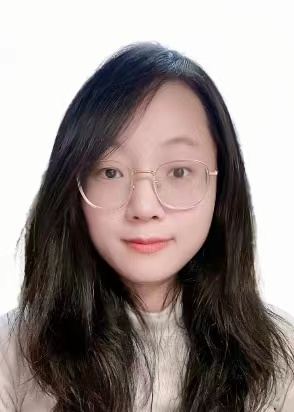
\includegraphics[width=1in,height=1.25in,clip,keepaspectratio]{Photos/xueli_sun.jpeg}}]{Xueli Sun}
         received the Ph.D. degree in computer science from Soochow University, Suzhou, China. She is currently a Lecturer with the School of Internet of Things, Nanjing University of Posts and Telecommunications. Her current research interests include interconnection architectures, data center networks, fault diagnosis, network reliability, and graph learning.
    \end{IEEEbiography}
\end{minipage}
\vspace{-5mm}
\begin{minipage}{0.45\textwidth}
    \begin{IEEEbiography}[{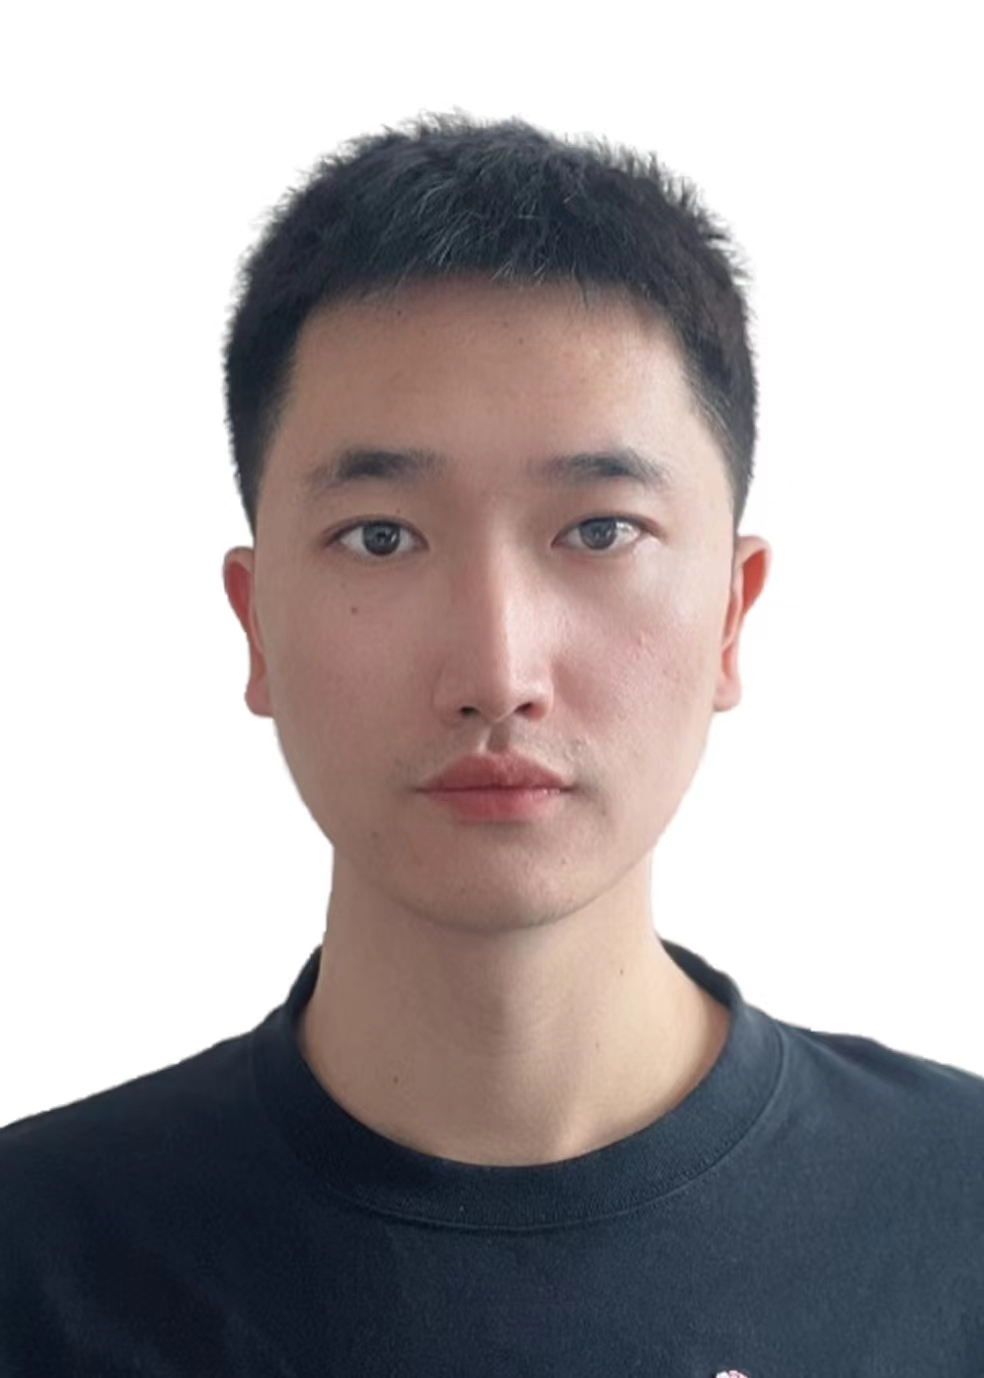
\includegraphics[width=1in,height=1.25in,clip,keepaspectratio]{Photos/shuangxiang_kan.jpeg}}]{Shuangxiang Kan}
        received the M.Sc. degree from Soochow University, in 2021. He is currently working toward the Ph.D. degree with the University of New South Wales. His current research interests include static and dynamic program analysis, program verification, and interconnection architectures.
    \end{IEEEbiography}
\end{minipage}
\vspace{-5mm}
\begin{minipage}{0.45\textwidth}
    \begin{IEEEbiography}[{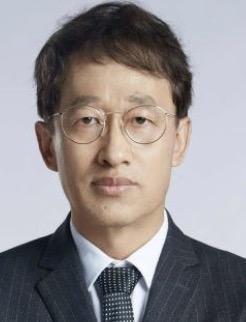
\includegraphics[width=1in,height=1.25in,clip,keepaspectratio]{Photos/jianxi_fan.jpeg}}]{Jianxi Fan}
        received the Ph.D. degree in computer science from the City University of Hong Kong, Hong Kong, in 2006. He is currently a Professor with the School of Computer Science and Technology, Soochow University, China.  His research interests include parallel and distributed systems, interconnection architectures, data center networks, and graph algorithms.
        % received the B.S. degree in computer science from Shandong Normal University, Jinan, in 1988, the M.S. degree in computer science from Shandong University, Jinan, in 1991, and the Ph.D. degree in computer science from the City University of Hong Kong, Hong Kong, in 2006. He is currently a Professor with the School of Computer Science and Technology, Soochow University, China.  His research interests include parallel and distributed systems, interconnection architectures, data center networks, and graph algorithms.
    \end{IEEEbiography}
\end{minipage}
\vspace{-5mm}
\begin{minipage}{0.45\textwidth}
    \begin{IEEEbiography}[{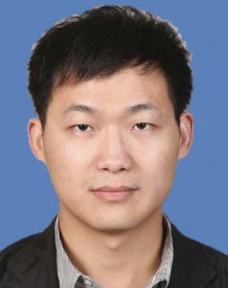
\includegraphics[width=1in,height=1.25in,clip,keepaspectratio]{Photos/weibei-fan.jpeg}}]{Weibei Fan}
        (Member, IEEE) received the Ph.D. degree in computer science from Soochow University, in 2019. He is currently an Associate Professor with the School of Computer, Nanjing University of Posts and Telecommunications. His research interests include data centers, parallel and distributed systems, and interconnection architectures.
    \end{IEEEbiography}
\end{minipage}
\vspace{-5mm}
\begin{minipage}{0.45\textwidth}
    \begin{IEEEbiography}[{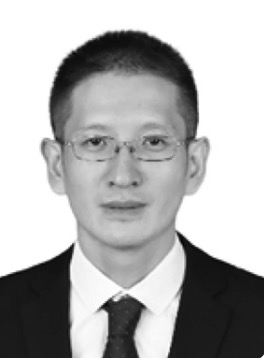
\includegraphics[width=1in,height=1.25in,clip,keepaspectratio]{Photos/jin_qi.jpeg}}]{Jin Qi}
        (Member, IEEE) received the Ph.D. degrees in information network from Nanjing University of Posts and Telecommunications, Nanjing, China, in 2012. He is currently a Professor with the School of Internet of Things in Nanjing University of Posts and Telecommunications. His main research interests are in the areas of intelligent computing, industrial Internet, and energy Internet.
    \end{IEEEbiography}
\end{minipage}
\vspace{-5mm}
\begin{minipage}{0.45\textwidth}
    \begin{IEEEbiography}[{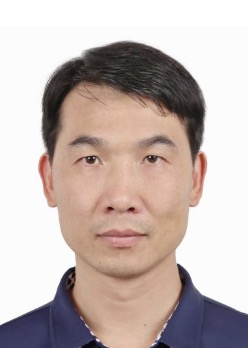
\includegraphics[width=1in,height=1.25in,clip,keepaspectratio]{Photos/zhenjiang_dong.jpeg}}]{Zhenjiang Dong}
         received the Ph.D. degree from Shanghai Jiao Tong University, Shanghai, China. He is currently a Full Professor with the School of Computer Science, Nanjing University of Posts and Telecommunications. His current research interests include security of data element flows, privacy computing, cyberspace security, and blockchain.
    \end{IEEEbiography}
\end{minipage}


\end{document}